%% analyse.tex
\chapter{Konzept}
\label{ch:Konzept}
%% ==============================
Dieses Kapitel befasst sich darum, welche Algorithmen in KNIME implementiert wurden und erklärt deren Vorgehensweise. Zuerst wird der Block Nested Loop \cite{borzsony2001skyline}, ein Skylinealgorithmus gezeigt. Die Skyline wird von manchen repräsentativen Skylinealgorithmen zur Berechnung benötigt. Daher ist mindestens ein Skylinealgorithmus für die Arbeit zwingend notwendig. Zur Bestimmung von repräsentativen Skylines wird in dieser Arbeit als erstes der DominationMaximizer \cite{4221657} vorgestellt. Dieser versucht die \textit{k} Skylinedatensätze heraus zu suchen, die die Anzahl der dominierten Datensätze maximieren. Der zweite vorgestellte Algorithmus basiert auf Distanz \cite{Tao:2009:DRS:1546683.1547325} und sucht die Repräsentanten heraus, sodass die Distanz zwischen einem Nicht-Repräsentanten und dem nächstliegendsten Repräsentanten minimal ist. Der letzte vorgestellte Algorithmus ist der E-Greedy \cite{magnani2014taking}. Das Ziel dieses ist es die repräsentative Skyline durch Berücksichtigung von Diversität und Signifikanz der Datensätze zu bestimmen.
Zum Schluss dieses Kapitels werden genauere Details zur Funktionsweise der drei wichtigen Klassen NodeModel, NodeDialog und NodeView von KNIME aufgeführt, die für die Implementierung der Algorithmen eine wichtige Rolle spielen.
%% ==============================
\section{Block Nested Loop}
\label{ch:Analyse:sec:skyAlgos}
%% ==============================
Methoden zur Berechnung einer Skyline gibt es viele, wie zum Beispiel Nested SQL Statements, Block-Nested-Loop, Divide \& Conquer, etc.
Zusätzlich gibt es auch viele Ansätze, die auf B/R-Bäume aufbauen, wie zum Beispiel der Algorithmus in \cite{Papadias:2003:OPA:872757.872814}. Der Vorteil bei diesen ist, dass sie während der Berechnung schon Datensätze der Skyline ausgeben können und im Fall von Suchabfragen dem User schon nach kurzer Zeit einige Ergebnisse liefern können. Weiterhin sind Algorithmen, die auf B/R-Bäumen basieren oft schneller als andere Algorithmen, da oft viele Vergleiche durch Pruning der Bäume oder mithilfe der Branch \& Bound Methode reduziert werden können. 
Da in dieser Arbeit der Mittelpunkt repräsentative Skyline sind, wurde für diese Arbeit nur der Block-Nested-Loop Algorithmus implementiert, da dieser intuitiv und für den Zweck dieser Arbeit ausreichend ist. Weitere Skyline-Algorithmen in KNIME einzubauen, wäre ein guter Schritt diese Arbeit fortzusetzen. 

Der Block-Nested-Loop Algorithmus basiert auf einer einfachen geschachtelten Schleife. Zur Reduzierung der Rechenzeit wurde ein Fenster $w$ eingeführt, in welchem unvergleichbare bzw. undominierte Datensätze gespeichert werden. Meistens bestimmt der User wie viele Datensätze im Fenster gespeichert werden können.
Beim Einlesen eines Datensatzes, wird er mit allen anderen Datensätzen in $w$ verglichen. Hier gibt es drei Möglichkeiten:
Falls der eingelesene Datensatz $p$ von einem oder mehreren Datensätzen in $w$ dominiert wird, wird er eliminiert und in folgenden Iterationen nicht mehr betrachtet. Dies führt zu großen Einsparungen der Rechenzeit. 
Falls $p$ jedoch einen oder mehrere Datensätze in $w$ dominiert, werden diese Datensätze von $w$ entfernt und $p$ wird zu $w$ hinzugefügt.
Bei Unvergleichbarkeit wird $p$ in $w$ eingefügt, falls in $w$ noch nicht die vom User bestimmte Grenze erreicht ist. Ansonsten wird $p$ in eine temporäre Datei geschrieben.

Die Datensätze in der temporären Datei werden in der nächsten Iteration mit dem Fenster verglichen. Dieser Vorgang wird so lange wiederholt bis nach einer Iteration kein Datensatz mehr in der temporären Datei vorhanden ist.
Damit dieser Vorgang terminiert, bekommen Datensätze beim Einfügen in $w$ oder in die temporäre Datei einen Zeitstempel. Beim Einlesen des Datensatzes, wird jeder Datensatz in $w$ mit einem geringeren Zeitstempel ausgegeben  bzw. in die Skyline eingefügt.
Weiterhin werden nach der ersten Iteration alle Datensätze aus $w$ zur Skyline hinzugefügt, bei der während des Hinzufügens in $w$ die temporäre Datei leer war.
Diese beiden Kriterien sorgen nicht nur für die sichere Terminierung des Algorithmus, sondern auch für eine Einsparung der Rechenzeit.
Ein Pseudo-Code für diesen Algorithmus befindet sich im Anhang von \cite{borzsony2001skyline}.

Da sich diese Arbeit hauptsächlich um repräsentative Skylines und Präferenzen befasst und trotzdem eine Implementierung eines Skylinealgorithmus erforderlich war, fiel die Entscheidung auf den Block-Nested-Loop. Dieser war einfach und schnell zu implementieren und liefert im Gegensatz zu einer normalen verschachtelten Schleife ein schnelleres Ergebnis.  
%% ==============================
\section{Repräsentative Skyline Algorithmen}
\label{ch:Analyse:sec:repSkyAlgos}
%% ==============================
In diesem Abschnitt des Kapitels werden die Algorithmen zur Berechnung einer repräsentativen Skyline, die für diese Arbeit in KNIME implementiert wurden, vorgestellt. 
Diese basieren hauptsächlich auf einen der zwei Ziele: Diversität oder Signifikanz zu maximieren (siehe Abschnitt \ref{ch:Grundlagen:sec:repSkyline}).
Zur Gegenüberstellung wurden sowohl Algorithmen implementiert, die den originalen Datensatz als Eingabe bekommen als auch welche, die nur mit einer Skyline als Eingabe arbeiten können.
%% ==============================
\subsection{DominationMaximizer}
\label{ch:Analyse:sec:repSkyAlgos:subsec:domMax}
%% ==============================
Der DominationMaximizer (Algorithmus \ref{algo:domMaximizer}) ist eine kleine Abwandlung des Greedy-Algorithmus, der in Kapitel 5.2 von \cite{4221657} vorgestellt wird. 
Das Ziel beider Algorithmen ist es $k$ Datensätze zu finden, die zusammen maximal viel andere Datensätze dominieren.

\begin{algorithm}[H]
\caption{DominationMaximizer}\label{algo:domMaximizer}
\begin{algorithmic}[1]
\INPUTBF $k$ int, $P$ set of data points
\OUTPUTBF $k$ skyline points
\State $S_P = \varnothing$ and $S = \varnothing$
\State \textbf{for each} data point $p$ in $P$ 
\State \hspace{\algorithmicindent} \textbf{for each} data point $q$ in $P$
\State \hspace{\algorithmicindent} \hspace{\algorithmicindent} \textbf{if} $p \succ q$ \textbf{then} 
\State \hspace{\algorithmicindent} \hspace{\algorithmicindent} \hspace{\algorithmicindent} $S_P:= S_P \cup \{p\}$ and $S_P:= S_P-\{q\}$
\State \hspace{\algorithmicindent} \hspace{\algorithmicindent} \hspace{\algorithmicindent} $D(\{p\}):=D(\{p\}) \cup \{q\}$  
\State \textbf{while} $|S|<k$ and $S_P-S \neq \varnothing$ \textbf{do}
\State \hspace{\algorithmicindent} choose $s \in {S_P-S}$ such that $|D(\{s\} \cup S)|$ is maximized
\State \hspace{\algorithmicindent} $S:=\{s\} \cup S$
\State \textbf{return} $S$
\end{algorithmic}
\end{algorithm}

Im Gegensatz zum Greedy-Algorithmus berechnet der DominationMaximizer Algorithmus die Skyline und die Menge der dominierten Datensätze für jeden undominierten Datensatz gleichzeitig. Falls bei einem Vergleich zwischen zwei Datensätzen einer der beiden vom anderen dominiert wird, wird der dominierte Datensatz der Menge $D$ des dominierenden Datensatzes hinzugefügt. $D\{s\}$ ist somit die Menge von Datensätzen, die von Datensatz $s$ dominiert werden. 

Der Greedy-Algorithmus legt nicht fest, welcher Algorithmus für die Berechnung der Skyline benötigt wird. Für den DominationMaximizer wird eine einfache verschachtelte Schleife verwendet, um sicher zu stellen, dass jeder Datensatz mit allen anderen verglichen wird. 
Nach dem Durchlaufen der Schleife werden $k$ Datensätze ausgewählt, die erstens von keinem anderen Datensatz dominiert werden und die die Menge an dominierten Datensätzen maximieren.

Das Problem dieses Algorithmus ist, dass bei Daten mit geringer Streuung und wenigen vorhandenen Ausreißer nur Skylinedatensätze, die nah an dominierten Datensätzen liegen, in der repräsentativen Skyline enthalten sind. Dies liegt daran, dass Skylinedatensätze, die nah an dominierten Datensätzen liegen, sehr wahrscheinlich in allen betrachteten Dimensionen besser sind als die dominierten und somit am meisten Datensätze dominieren.  Da Ausreißer meistens nur undominierten Datensätzen entsprechen, die keinen anderen Datensatz dominieren, werden diese meistens vom DominationMaximizer nicht zur Skyline hinzugefügt. Dies hat zur Folge, dass die Repräsentationsgüte für solche Fälle relativ niedrig ist, da Ausreißer dadurch nie in der repräsentativen Skyline enthalten sind, was gut in Abbildung \ref{img:dominationMaximizerGraph} zu sehen ist.
 
\begin{figure}[H]
	\centering
	\includegraphics[width=\textwidth]{dominationMaximizerGraph.png}
	\caption{Die repräsentative Skyline des DominationMaximizer bei Daten mit hoher Dichte}
	\label{img:dominationMaximizerGraph}
\end{figure}
%% ==============================
\subsection{Distanz-basierende repräsentative Skyline}
\label{ch:Analyse:sec:repSkyAlgos:subsec:disBasedRepSky}
%% ==============================
Angenommen die Menge $S$ beinhaltet alle Skylinedatensätze und $K$ entspricht einer repräsentativen Skyline mit $k$ Datensätzen. Mit diesen beiden Mengen kann nun der repräsentative Fehler $Er(K,S)$ berechnet werden. 
$$Er(K,S)=\max\limits_{p\in{S-K}}\{\min\limits_{p^{'} \in{K}}||p,p^{'}||\}$$
Entsprechend dieses Fehlers ist eine repräsentative Skyline gut, falls für jeden nicht repräsentativen $\in{S-K}$, ein repräsentativer $\in{K}$ in der Nähe ist. An der Formel ist zu erkennen, dass der Fehler die Repräsentationsgüte anhand der Distanz zwischen einem nicht-repräsentativen Datensatz und dem nächstliegenden repräsentativen Datensatz misst. Diese Distanz wird mit der euklidischen Distanz berechnet.
Das Ziel des Algorithmus ist es die $k$ Datensätze zu finden, mit denen dieser repräsentative Fehler minimal ist. Bedingung für die korrekte Durchführung des Algorithmus sind, dass alle Datensätze nur zwei Dimensionen besitzen oder nur zwei betrachtet werden. Zusätzlich sollten die Datensätze nach der ersten Dimension aufsteigend sortiert werden. Für dieses Arbeit wird der Algorithmus in KNIME implementiert und dadurch wird die Sortierung im entsprechenden KNIME Node durchgeführt, damit sich der User damit nicht befassen muss. 

Die Funktion $opt(i,t)$ bestimmt die $t$ große optimale repräsentative Skyline von $S_i$, wobei $t \leq i$ gilt. $S_i$ ist hier eine Teilmenge von $S$ mit $i \leq m$ (m=Anzahl der Skylinedatensätze). Falls $i=m$ und somit $S_i=S$ gilt, entspricht $opt(m,k)$ der optimalen $k$ großen repräsentativen Skyline von $S$.
Um diese Funktion jedoch berechnen zu können, muss zuerst der optimale Repräsentationsfehler von $opt(i,t)$ bestimmt werden.
$$optEr(i,t)=\min\limits_{j=t}^{i-1}\{max\{optEr(j-1,t-1),radius(j,i)\}\}$$
Die Werte von $i$,$j$ und $t$ entsprechen den Indizes von Datensätzen der Skyline. Diese Formel bestimmt rekursiv die $t$ kleinsten Radien beziehungsweise die $t$ kleinsten Kreise, die zusammen alle $m$ Datensätze umfassen. Es ist zu erkennen, dass der repräsentative Fehler dem niedrigsten Radius entspricht, der die meisten Datensätze umfasst.

Angenommen $v$ sei der Wert von $j$ bei dem oben genannte Funktion $optEr(i,t)$ ihr Minimum findet\footnote{Die Indizes der beiden Funktionen müssen hierbei identisch sein. Für $opt(8,3)$ wird der Wert von $j$ für $v$ verwendet, bei der die Funktion $optEr(8,3)$ ihr Minimum erreicht.}, dann ergibt sich die repräsentative Skyline durch folgende Funktion:
$$opt(i,t)=opt(v-1,t-1)\cup\{center(v,i)\}$$
Diese Funktion wird wie $optEr(i,t)$ rekursiv berechnet und fügt die Datensätze hinzu, die Mittelpunkte der Kreise sind, die alle $i$ Datensätze umfassen. Dadurch das $v$ der Wert von $j$ ist, bei der die Funktion $optEr(i,t)$ ihr Minimum erreicht, wird erzwungen das nur Kreise betrachtet werden, die mit geringem Radius die meisten Datensätze umfassen.   
Für die Berechnung der umfassenden Kreisradien, wird die euklidische Distanz benutzt:
$$radius(i,j)=\min\limits_{u=i}^{j}\{max\{||p_i,p_u||,||p_u,p_j||\}\}$$
Der Punkt $p_u=center(i,j)$ bei dem diese Funktion ihr Minimum erreicht, ist der Mittelpunkt des Kreises, der alle Datensätze zwischen den Datensätzen bei Index $i$ und $j$ umfasst.

\begin{algorithm}[H]
\caption{2D-opt ($S$,$k$)}\label{algo:2DOpt}
\begin{algorithmic}[1]
\INPUTBF the skyline $S$ of dataset $D$ and an integer $k$
\OUTPUTBF the representative skyline of $D$
\State \parbox[t]{\dimexpr\linewidth-\algorithmicindent}{\textbf{for each} pair of $(i,j)$ such that $1 \leq i \leq j \leq m$, derive\par 
$radius(i,j)$ and $center(i,j)$\strut}
\State \parbox[t]{\dimexpr\linewidth-\algorithmicindent}{set $opt(i,1) = \{center(1,i)\}$ and $optEr(i,1)=radius(1,i)$\par
\textbf{for each} $1 \leq i \leq m$\strut}
\State \textbf{for} $t=2$ \textbf{to} $k-1$
\State \hspace{\algorithmicindent} \textbf{for} $i=t$ \textbf{to} $m$
\State \hspace{\algorithmicindent}\hspace{\algorithmicindent} compute $optEr(i,t)$
\State \hspace{\algorithmicindent}\hspace{\algorithmicindent} compute $opt(i,t)$
\State compute $optEr(m,k)$ and $opt(m,k)$
\State \textbf{return} $opt(m,k)$
\end{algorithmic}
\end{algorithm}

Algorithmus \ref{algo:2DOpt} berechnet zuerst alle wichtigen Werte, die für die $k$ repräsentative Skyline mit $m$ Skylinedatensätzen benötigt wird. Zeile $2$ dient dazu, dass sowohl $opt(i,t)$ als auch $optEr(i,t)$ terminieren. Das Paper \cite{Tao:2009:DRS:1546683.1547325} dieses Algorithmus berechnet in Zeile $7$ die Funktionen $optEr(k,m)$ und $opt(k,m)$ und nicht $optEr(k,m)$ und $opt(k,m)$. Dies hätte zur Folge, dass für die Berechnung der Formeln $i$ kleiner als $t$ ist und es somit nie zu einem Ergebnis kommen würde.
Das Ergebnis von $opt(m,k)$ kann als repräsentative Skyline ausgegeben werden und dem Kunden präsentiert werden.

Der Algorithmus basiert nur auf Diversität und versucht Datensätze, die möglich weit voneinander entfernt sind zu finden, um damit alle möglichen Cluster der Skyline repräsentieren zu können. Der Algorithmus im nächsten Abschnitts versucht diesen Ansatz zu erweitern und berücksichtigt zusätzlich die Signifikanz von Datensätzen, falls diese gegeben sind.  
%% ==============================
\subsection{E-Greedy}
\label{ch:Analyse:sec:repSkyAlgos:subsec:eGreedy}
%% ==============================
Der E-Greedy Algorithmus \cite{magnani2014taking} versucht nicht nur die Diversität von Datensätzen zu maximieren, sondern auch gleichzeitig die Signifikanz zu beachten.
Signifikanz wird dadurch bestimmt, indem der User für jede Dimension seiner Wahl einen Thresholdwert oder ein Thresholdintervall angibt. Die Datensätze, die entweder den Thresholdwert übersteigen bzw. unter diesem liegen oder in dem entsprechenden Intervall liegen, sind signifikant. Bei fehlenden Thresholds einer Dimension werden alle Datensätze bei alleiniger Betrachtung dieser Dimension als gleich signifikant gesehen. Dieser Ansatz kann noch erweitert werden, indem Thresholds durch vergangene Daten bestimmt werden. 

$$\text{Representative Skyline} = \argmax{S \in{P_k(sky(R))}} obj(S)$$

$obj(S)$ ist hier eine Funktion, die die Werte der Diversität und Signifikanz darstellt. $P_k(sky(R))$ ist eine Teilmenge mit $k$ Datensätzen der Skyline. Somit entspricht die repräsentative Skyline der Teilmenge, bei der die Funktion $obj(S)$ ihr Maximum erreicht.

$$\lambda \sum\limits_{r \in{S \backslash \{r\}}} min_{s \in S \backslash \{r\}}\delta(r,s)+(1- \lambda) \sum\limits_{r \in{S}}E(\sigma(r))$$

Die Funktion $obj(S)$ besteht aus zwei Teilen. Der Signifikanz $\sigma$ und der Diversität $\delta$.
Mit einem Gewichtungsfaktor $\lambda$ kann der User bestimmen, welcher der beiden Aspekte ihm wichtiger ist. Anzumerken ist, dass der \textbf{erwartete} Wert der Signifikanz $\sigma(r)$ berechnet wird. 

$$\begin{displaystyle}
  I_i(r, s) = \left.
  \begin{cases}
    0 & \text{if } r=s \\
    \frac{|\{o \in{sky(R)}| (r.i \geq o.i \geq s.i) \lor (s.i \geq o.i \geq r.i)\}|-1}{|sky(R)|-1} & \text{if } r \neq s
  \end{cases}
  \right.
\end{displaystyle}$$

Um die Diversität zu berechnen, wird für jede Datensatzkombination und jede Dimension $i$ die Anzahl von Skylinedatensätzen, die zwischen zwei Datensätzen liegt, gezählt. Da $I_i$ dem relativen Anteil der dazwischen liegenden Punkte entsprechen soll, wird durch die $\text{Anzahl aller Skylinedatensätze}-1$ geteilt.

$$\delta_{sed}(r,s)=\frac{\sum\limits\mathop{}_{\mkern-5mu i \in{[1,d]}} I_i(r,s)}{d}$$

Durch das Summieren aller $I_i$, geteilt durch die Anzahl der Dimensionen, entsteht schlussendlich die Diversität bzw. den Wert wie sehr die Datensätze $r$ und $s$ voneinander abweichen. Diesen Wert zu maximieren führt dazu, dass die Anzahl der Datensätze zwischen zwei Datensätzen maximal sein sollte. Dadurch enthält die repräsentative Skyline bei alleiniger Betrachtung von Diversität nur Datensätze, die weit voneinander entfernt sind. 

$$\sigma_{sss}(r)=\frac{logit(r)}{max\mathop{}_{\mkern-5mu s \in{sky(R)}}logit(s)}$$

Da die Thresholds durch einen User bestimmt werden, wird die für die Berücksichtigung der Signifikanz die Sigmoid Funktion benutzt, da diese User Präferenzen repräsentieren kann. Die Skyline Sigmoid Signifikanz $\sigma_{sss}$ ergibt sich durch die logistische Sigmoid Funktion des betrachteten Datensatzes geteilt durch die logistische Sigmoid Funktion des Datensatzes, der von allen Datensätzen den höchsten Wert für die logistische Sigmoid Funktion besitzt. Die logistische Sigmoid Funktion wird je nachdem, ob der Benutzer einen einzelnen Thresholdwert oder ein Thresholdintervall eingegeben hat, anders berechnet.

Wie oben genannt wird eine Eingabe eines Thresholds für die Berechnung der Signifikanz benötigt. Bei der Eingabe eines einzelnen Wertes, hier $t$ genannt, wird die logistische Sigmoidfunktion wie folgt bestimmt:

$$logit(r)=\frac{\sum\mathop{}_{\mkern-5mu i \in{[1,d]}\frac{1}{1+e^{-r.i+t.i}}}}{d}$$

Zur Berechnung der logistischen Sigmoidfunktion  wird $\frac{1}{1+e^{-r.i+t.i}}$ für alle Dimension summiert, wobei $r.i$ der Wert von Dimension $i$ des entsprechenden Datensatzes $r$ entspricht. $t.i$ entspricht dagegen dem Wert des Thresholds für diese Dimension. Diese Funktion wird benutzt falls der Threshold als untere Grenze benutzt wird und alle Datensätze mit Werten über diesem Threshold als signifikant gesehen werden. 
Es wird angenommen, dass der User ein Auto mit einer PS-Leistung von 100 oder mehr bevorzugt. Aus dieser Angabe würde sich für $\frac{1}{1+e^{-r.i+t.i}}$ der Funktionsgraph in Abbildung \ref{img:logitFunction} ergeben. Es ist gut zu erkennen, dass bei einem Wert von 100 die Signifikanz bei $50\%$ liegt und somit bei einer reinen Betrachtung der PS-Leistung jedes Auto mit einer höheren PS-Leistung als signifikant gesehen wird.

\begin{figure}[H]
	\centering
	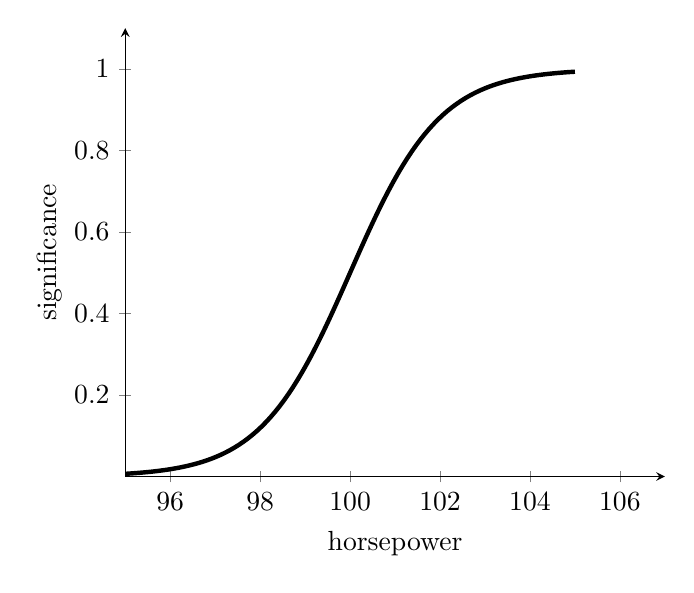
\begin{tikzpicture}
	\begin{axis}[
    axis lines=middle,
    xmax=107,
    xmin=95,
    ymin=0,
    ymax=1.1,
     x label style={at={(axis description cs:0.5,-0.1)},anchor=north},
    y label style={at={(axis description 	cs:-0.1,.5)},rotate=90,anchor=south},
    xlabel={horsepower},
    ylabel={significance}
    ]
    \addplot [domain=95:105, samples=100, ultra thick, black] {1/(1+e^(-	x+100))};
    \vasymptote {100}
	\end{axis}
\end{tikzpicture}
	\caption{Die Funktion $\frac{1}{1+e^{-r.i+t.i}}$ bei einem Thresholdwert von 100}
	\label{img:logitFunction}
\end{figure}

Falls jedoch der Threshold als obere Grenze genommen wird, ändert sich die Funktion wie folgt:

$$logit(r)=\frac{\sum\mathop{}_{\mkern-5mu i \in{[1,d]}\frac{1}{1+e^{r.i-t.i}}}}{d}$$

Für Thresholdintervalls sind diejenigen Datensätze signifikant, dessen Werte in dem Intervall liegen. Die dazugehörige Logit-Funktion wird wie folgt berechnet:
$$logit(r)=\frac{\sum\limits\mathop{}_{\mkern-5mu i \in{[1,d]}}\frac{1}{b.i-a.i}(-ln(1+e^{(r-i-b.i)})+ln(1+e^{(r.i-a.i)}))}{d}$$

$a.i$ entspricht hier der unteren Grenze und $b.i$ der obere Grenze des Thresholdintervalls. 


Nach der Berechnung der Signifikanz und der Diversität, kann die endgültige Objektfunktion bestimmt werden, die hier $\bar{\delta}$ genannt wird.
$$\bar{\delta}(r,s)= \lambda \text{ } \delta(r,s)+(1- \lambda)E(\sigma(r))$$

Um nun die $k$ repräsentativen Skylinedatensätzen zu bestimmen, die diese Objektfunktion maximieren, wird der Algorithmus \ref{algo:eGreedy} benutzt. 


\begin{algorithm}[H]
\caption{E-Greedy}\label{algo:eGreedy}
\begin{algorithmic}[1]
\INPUTBF $S$ skyline, $k$ int
\State RS $:=$ emptylist
\State RS $\leftarrow$ most significant record in $S$
\State \textbf{for} $i: 1\ldots k-1$ \textbf{do}
\State \hspace{\algorithmicindent}r = $arg$ $max_{r\in{S}}$ $\bar{\delta}(r,RS)$
\State \hspace{\algorithmicindent} RS $\leftarrow$ r
\State \textbf{end for}
\State \textbf{return} RS
\end{algorithmic}
\end{algorithm}

Der erste Datensatz der zur repräsentativen Skyline hinzugefügt wird, ist der Datensatz mit der höchsten Signifikanz. Falls mehrere die gleiche Signifikanz besitzen, wird ein Datensatz von diesen zufällig ausgewählt.
Anschließend werden $k-1$ Datensätze hinzugefügt, die mit der bereits berechneten repräsentativen Skyline die Objektfunktion maximieren.

Der Vorteil des E-Greedy liegt darin, dass er sowohl Signifikanz als auch Diversität betrachtet. Andere Ansätze zur Berechnung von repräsentativen Skylines beruhen meistens nur auf einer der beiden Kriterien.  
\enquote{Existing approaches have only focused on partial aspects of this problem. Some try to identify sets of diverse records giving an overall approximation of the skyline. [...] Others exploit some knowledge of the record scoring function to identify the most significant record, but not sets of records representative of the whole skyline.} \cite[p. 1]{magnani2014taking}
 
Die Signifikanz den User bestimmen zu lassen, liefert eine repräsentative Skyline für seine Präferenzen entsprechend. Falls nun noch die Diversität betrachtet wird, können auch Ausreißer und die Verschiedenheit von Datensätzen berücksichtigt werden. Dies ermöglicht auch repräsentative Skylines zu berechnen für die der User nur bei bestimmten Dimensionen Thresholds festlegen kann.
Der Nachteil dieses Algorithmus ist, dass der Gewichtungsfaktor $\lambda$ die repräsentative Skyline stark verändert und der User oft nicht weiß wie er die Diversität und die Signifikanz gegeneinander gewichten soll. Dies bedeutet, dass es dazu kommen kann, dass die repräsentative Skyline mehr als nur einmal berechnet wird, um ein zufrieden stellendes Ergebnis zu finden.
%% ==============================
\section{KNIME}
\label{ch:Analyse:sec:knime}
%% ==============================
Wie schon in Abschnitt \ref{ch:Grundlagen:sec:knime} erwähnt, wird für die Implementierung KNIME benutzt. Ein Node in KNIME besteht aus mehreren wichtigen Klassen, die in diesem Kapitel vorgestellt werden.
%% ==============================
\subsection{NodeModel}
\label{ch:Analyse:sec:knime:subsec:nodeModel}
%% ==============================
Das NodeModel ist dafür zuständig den Algorithmus auszuführen und wichtige Daten intern zu speichern. 
Weiterhin wird überprüft, ob die Eingaben des Nodes die korrekten Datentypen besitzen und nicht leer sind.
Eingaben können zum Beispiel Datenbankverbindungen oder Datentabellen, in KNIME BufferedDataTables genannt, sein. Falls die Eingaben inkorrekt sind, kann eine Exception geworfen werden, die dem User einen Fehler anzeigt (siehe \ref{img:nodeModelError}).

\begin{figure}[H]
	\centering
	\includegraphics[width=\textwidth]{nodeModelError.png}
	\caption{Fehleranzeige eines Nodes}
	\label{img:nodeModelError}
\end{figure}

Es kann zusätzlich überprüft werden, ob mit den Eingaben der Algorithmus des Nodes durchführbar ist. Falls ein Algorithmus nur mit numerischen Werten arbeitet, kann überprüft werden, ob einzelne Datenspalten eines BufferedDataTables nur numerische Daten enthalten.

Nach Überprüfung der Eingaben werden diese dem auszuführenden Algorithmus übergeben, der daraufhin entsprechende Ausgaben zurück gibt. Weiterhin werden im NodeModel Meta Informationen zu den Ausgaben erstellt, um einen schnellen Zugriff auf Informationen wie Datenspaltennamen zu gewährleisten.

NodeModels können SettingsModels besitzen, die die Eingaben des Users im NodeDialog speichern. Die Wert dieser SettingsModels können für den Algorithmus oder dem NodeView verwendet werden. Das NodeModel besitzt auch Methoden, die zur Speicherung bestimmter Variablen und der genannten SettingModels benötigt werden, um diese beim Wiederöffnen von KNIME zu laden.
%% ==============================
\subsection{NodeDialog}
\label{ch:Analyse:sec:knime:subsec:nodeDialog}
%% ==============================
Diese Klasse dient dazu dem User eine Möglichkeit zu bieten, bestimmte Parameter für den Algorithmus selbst einstellen zu können. 
Dazu können entweder Standardkomponenten von KNIME verwendet werden oder es wird eine eigene graphische Oberfläche dem NodeDialog hinzugefügt.

Um diese Parameter der NodeModel Klasse und somit dem Algorithmus zu übergeben, werden die vorher erwähnten SettingModels benutzt. Diese können mit einem speziellen Schlüssel im NodeModel geladen werden.
Es können aber auch Variablen mit primitiven Datentypen durch die entsprechenden Methoden des NodeDialogs gespeichert und daraufhin im NodeModel zugegriffen werden.

In Abbildung \ref{img:nodeDialog} ist ein Beispiel des NodeDialogs des Database Connector Nodes zu sehen, für den eine Datenbank URL, ein JDBC Treiber und weitere Eingaben eingegeben werden können, um eine Datenbankverbindung aufzubauen.

\begin{figure}[H]
	\centering
	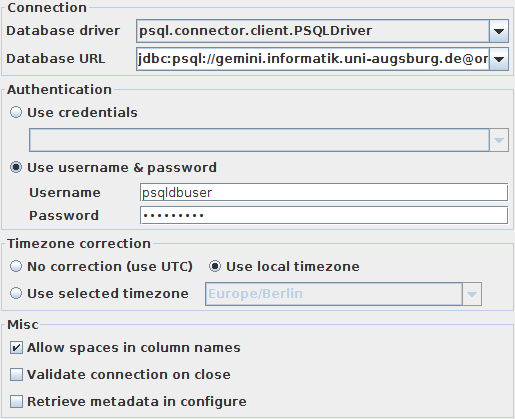
\includegraphics{nodeDialog.png}
	\caption{NodeDialogs des Database Connector Nodes}
	\label{img:nodeDialog}
\end{figure}

%% ==============================
\subsection{NodeView}
\label{ch:Analyse:sec:knime:subsec:nodeView}
%% ==============================
Die letzte Klasse, die von großer Relevanz ist, erzeugt eine Darstellung der Ein- oder Ausgaben. Die Darstellung kann je nach Ein- oder Ausgaben variieren (Histogramme, Koordinatensysteme mit Datenpunkten, Pie Charts, etc.).
Da der View eines Nodes nicht gespeichert wird, muss er bei jedem Öffnen von KNIME neu erzeugt werden.
Deswegen gibt es Methoden im NodeModel, die die Daten, die zur Erzeugung des Views benötigt werden in einer externen Datei speichern. Wie die SettingModels werden interne Dateien mit einem speziellen Schlüssel gespeichert und geladen. Im Gegensatz zur Kommunikation zwischen NodeModel und NodeDialog ist es möglich im NodeView durch Getter Methoden auf die Variablen der NodeModel Klasse zurückzugreifen. 

In Abbildung \ref{img:nodeView} ist ein Beispiel View des Histogramm Nodes zu sehen, der als Eingabe einen BufferedDataTable bekommt und nach Auswahl bestimmter Dimensionen ein Histogramm zeigt. 

\begin{figure}[H]
	\centering
	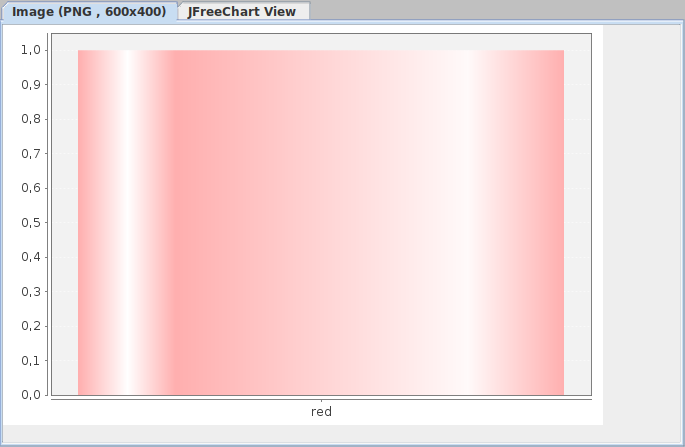
\includegraphics[width=\textwidth]{nodeView.png}
	\caption{Beispiel View des Histogramm Nodes}
	\label{img:nodeView}
\end{figure}

Nähere Informationen zur Funktionsweise und Implementierung von Nodes können auf der Webseite\footnote{https://tech.knime.org/developers (28.10.2016)} und dem Paper \cite{BCDG+07} von KNIME gefunden werden.
%% ==============================
%%% End: 
